\documentclass[12px]{article}
\setlength{\parindent}{4em}
\usepackage[margin=2cm]{geometry}
\usepackage{graphicx}
\usepackage{amsmath}
\usepackage{amssymb}
\usepackage{enumerate}
\usepackage{multicol}
\usepackage{color}
\usepackage[font=small,labelfont=bf]{caption}
\usepackage{pifont}
\usepackage{subcaption}
\usepackage{float}
\linespread{1.5}
\begin{document}
\begin{center}
    \Large\textbf{Vector, Geometry of Space and Coorodinate}\\
\end{center}
\begin{center}
    \textbf{"You had studied in high school, right?" (Prof. Duc-Thang Vo, 2023)}
\end{center}

\begin{enumerate}
    \item Coordinate
    \begin{enumerate}[(1)]
        \item Cartesian Coordinate:\\
            There are 2/3 mutually perpendicular directions in the 2D/3D Cartesian Coordinate.\\
            We will represent point P as $P(x,\ y,\ z)$.
            \begin{center}
                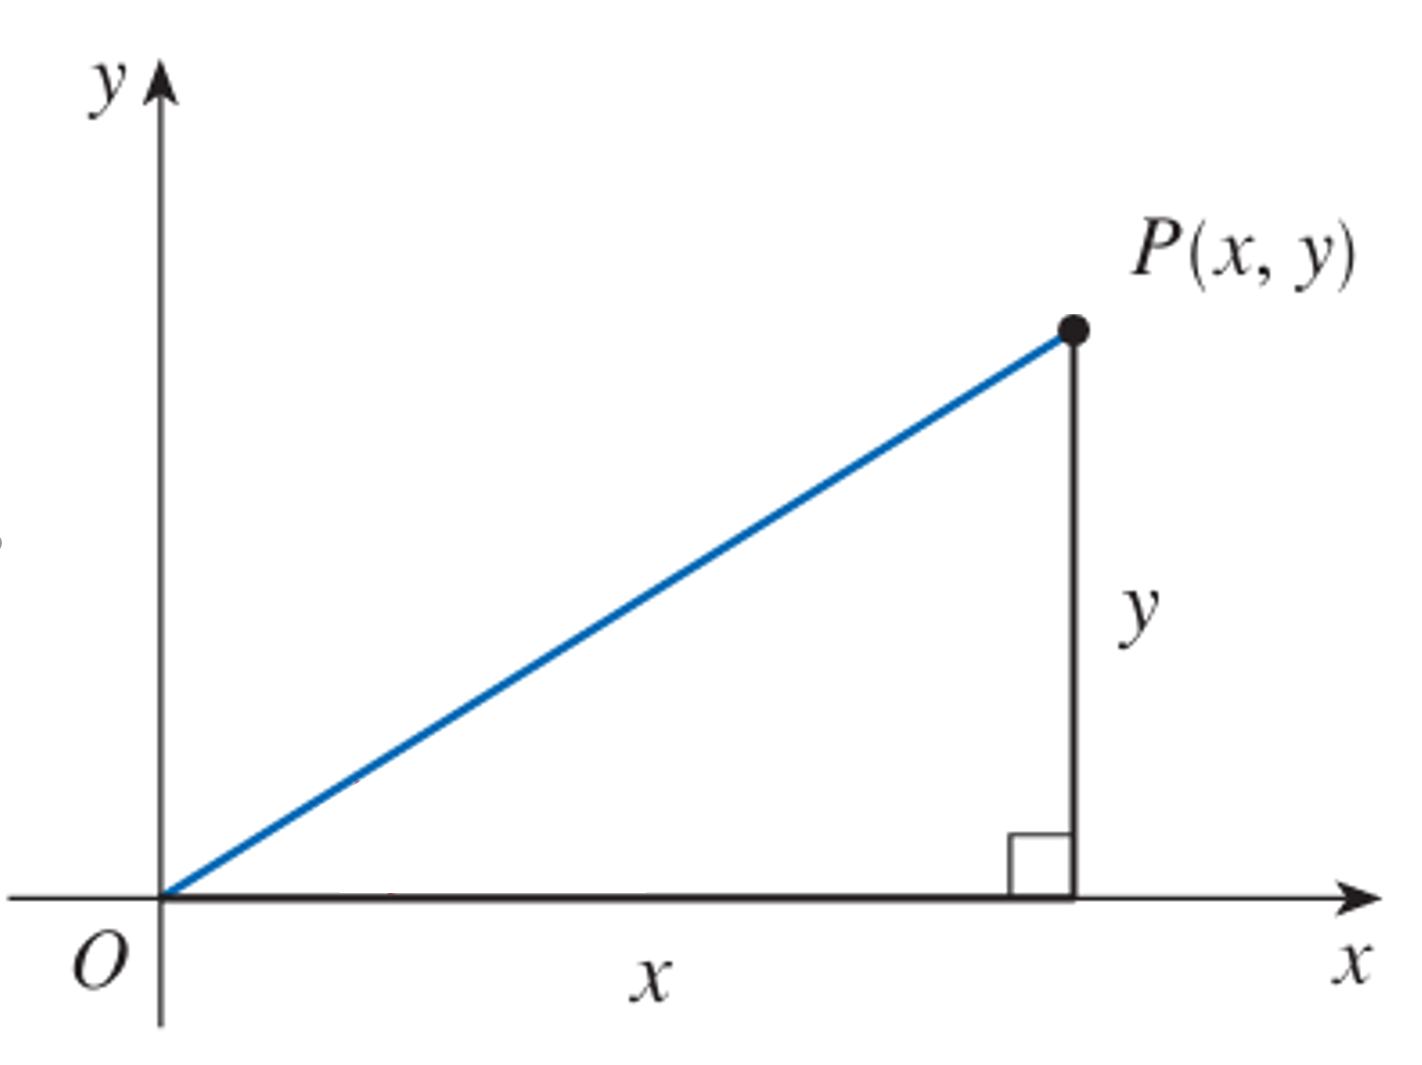
\includegraphics[width=5cm]{Cartesian.png}
            \end{center}
        \item Polar (Cylindrical) Coordinate:\\
            There are 1 length and 1 angle in the 2D Polar Coordinate. Adding a Z-axis will turn into Cylindrical coordinates.\\
            We will represent point P as $P(r,\ \theta,\ z)$.
            \begin{center}
                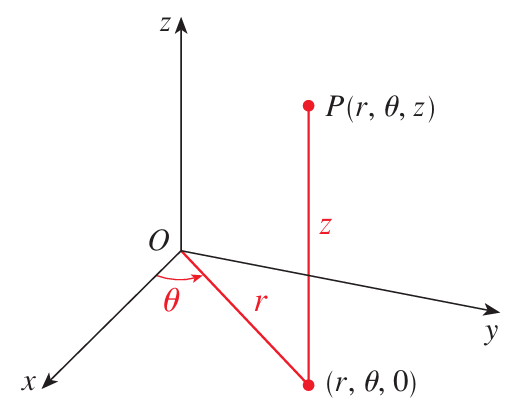
\includegraphics[width=5cm]{Cylindrical.png}
            \end{center}
        \item Spherical Coordinate:\\
        There are 1 length and 2 angles in the Spherical Coordinate.\\
        We will represent point P as $P(\rho,\ \theta,\ \phi)$.
        \begin{center}
            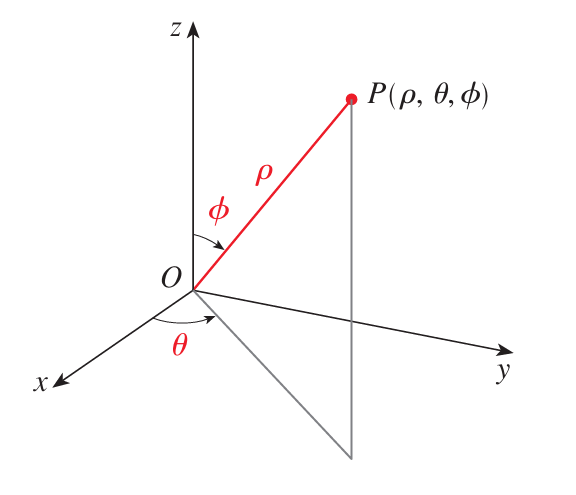
\includegraphics[width=5cm]{Sphere.png}
        \end{center}
    \end{enumerate}
\newpage
    \item Vector and Vector Algebra
    \begin{enumerate}[(1)]
        \item Scalar and Vector
        \begin{enumerate}
            \item Scarlar: Only has magnitude.
            \item Vector: Has both magnitude and direction 
        \end{enumerate}
        \item Representation of Vector:\\
        We usually use the bold font "$\textbf{v}$" or superscript arrow "$\overrightarrow{v}$" to represent the vector v. 
        \begin{enumerate}
            \item Tuple notation: $\textbf{v}=<v_1,\ v_2,\ \dots,\ v_n>$, and $n$ is finite integer.
            \item Matrix notation: $\textbf{v}=\begin{bmatrix}
                v_1\\v_2\\ \vdots\\v_n
            \end{bmatrix}$, and $n$ is finite integer.
        \end{enumerate}
        \item Basic Operations of Vector
        $$\textbf{v}=<v_1,\ v_2,\ \dots,\ v_n>,\ \textbf{u}=<u_1,\ u_2,\ \dots,\ u_n>$$
        \begin{enumerate}
            \item Addition and Subtraction:
            $$\textbf{v}+\textbf{u}=<v_1+u_1,\ v_2+u_1,\ \dots,\ v_n+u_n>$$
            $$\textbf{v}-\textbf{u}=<v_1-u_1,\ v_2-u_1,\ \dots,\ v_n-u_n>$$
            \item Scarlar Multiplication: 
            $$k\textbf{v}=<kv_1,\ kv_2,\ \dots,\ kv_n>$$
            \item Inner Product: (Scalar)\\
            Geometry Meaning: $v \cdot u\ =\ (v$'s Projection Length on $u$)*($u$'s Length)
            $$\textbf{v}\cdot\textbf{u}=v_1u_1+v_2u_2+ \dots +v_nu_n$$
            or we can use row vectors to calculate:
            $$\textbf{v}\cdot\textbf{u}=\textbf{v}^T\textbf{u}$$
            $$\textbf{v}^T\textbf{u}=
            \begin{bmatrix}v_1 &v_2 &\dots &v_n\end{bmatrix}\begin{bmatrix}u_1\\u_2\\ \vdots\\u_n\end{bmatrix}=
            \begin{bmatrix}
                v_1u_1+v_2u_2+ \dots +v_nu_n
            \end{bmatrix}=(Scalar)$$
            
\newpage
            \item Cross Product: (Vector)\\
            Geometry Meaning: 
            $\left\{\begin{aligned}
                &\ \textbf{v}\times\textbf{u}\perp\textbf{v}\ \text{and}\ \textbf{u}\ (\text{Perpendicular or Orthogonal})\\
                &\ |\textbf{v}\times\textbf{u}|=(\text{Area of Parallelogram expand by} \textbf{v} \text{and} \textbf{u}.)
            \end{aligned}\right.$
            $$\textbf{v}\times\textbf{u}\ =\ \begin{vmatrix}
                \hat{x_1} &\hat{x_2} &\hdots &\hat{x_n}\\
                v_1 &v_2 &\hdots &v_n\\
                \vdots &\vdots &\ddots &\vdots\\
                u_1 &u_2 &\hdots &u_n\end{vmatrix}\ =\ (Vector)$$
            \item Triple Product: (Volume $\rightarrow$ Scalar)\\
            $$\textbf{a}\cdot(\textbf{b}\times\textbf{c})=\textbf{c}\cdot(\textbf{a}\times\textbf{b})=\textbf{b}\cdot(\textbf{c}\times\textbf{a})=\begin{vmatrix}
                a_1&a_2&a_3\\
                b_1&b_2&b_3\\
                c_1&c_2&c_3
            \end{vmatrix}$$
            \item Outer Product: (Matrix)
            $$\textbf{v}\otimes\textbf{u}=\textbf{v}\textbf{u}^T$$
            $$\textbf{v}\textbf{u}^T=\begin{bmatrix}v_1\\v_2\\ \vdots\\v_n\end{bmatrix}
            \begin{bmatrix}u_1 &u_2 &\dots &u_n\end{bmatrix}=
            \begin{bmatrix}
                v_1u_1 &v_1u_2 &\hdots &v_1u_n\\
                v_2u_1 &v_2u_2 &\hdots &v_2u_n\\
                \vdots &\vdots &\ddots &\vdots\\
                v_nu_1 &v_nu_2 &\hdots &v_nu_n\\
            \end{bmatrix}$$
        \end{enumerate}
        \item Geometry of Space
        \begin{enumerate}
            \item Equation of Plane in $\mathbb{R}^3$.\\
            If the normal vector of the plane is $<a,\ b,\ c>$, and the plane passes through point $P(x_0,\ y_0,\ z_0)$, then the equation of the plane is
            $$E:\ a(x-x_0)+b(y-y_0)+c(z-z_0)=0$$
            or we can use the intercept form
            $$\frac{x}{x_i}+\frac{y}{y_i}+\frac{z}{z_i}=1$$
            $x_i,\ y_i,\ z_i$ are the intercepts of the plane with each axis.
            \item Equation of Line in $\mathbb{R}^3$.
            If the direction vector of the line is $<a,\ b,\ c>$, and the line passes through point $P(x_0,\ y_0,\ z_0)$, then the equation of the line is
            $$L:\ \frac{x-x_0}{a}=\frac{y-y_0}{b}=\frac{z-z_0}{c}\ (abc\neq 0)$$
            or we can use the parametric form
            $$L:\ \left\{\begin{aligned}
                x=at+x_0\\
                y=bt+y_0\\
                z=ct+z_0
            \end{aligned}\right.\ (t\in\mathbb{R})$$
        \end{enumerate}
\newpage
        % \item Linear Dependence/Independence\\
        % For several vector $\textbf{a}_1,\ \textbf{a}_2,\ \textbf{a}_3,\ ...,\ \textbf{a}_n$, if there exist a non-trivial solution such that \\$c_1\textbf{a}_1+c_2\textbf{a}_2+c_3\textbf{a}_3+...+c_n\textbf{a}_n=\textbf{0}$, they are said linear dependent.\\
        % To determine whether the set of the vectors is linear independent, we can use the Gauss Elimination:\\
        % \\
        % For example,
        % $$\begin{bmatrix}v_1\\v_2\\v_3\\v_4\end{bmatrix}=
        % \begin{bmatrix}
        %     1&1&-1&0\\
        %     2&2&1&-4\\
        %     0&3&-2&1\\
        %     3&6&1&-7
        % \end{bmatrix}$$
        % Processing with Gauss Elimination (Using Elementary Matrix):
        % $$
        % \begin{bmatrix}
        %     1&0&0&0\\
        %     -2&1&0&0\\
        %     0&0&1&0\\
        %     -3&0&0&1
        % \end{bmatrix}
        % \begin{bmatrix}
        %     1&1&-1&0\\
        %     2&2&1&-4\\
        %     0&3&-2&1\\
        %     3&6&1&-7
        % \end{bmatrix}=
        % \begin{bmatrix}
        %     1&1&-1&0\\
        %     0&0&3&-4\\
        %     0&3&-2&1\\
        %     0&3&4&-7
        % \end{bmatrix}$$
        % $$
        % \begin{bmatrix}
        %     1&0&0&0\\
        %     0&1&0&0\\
        %     0&0&1&0\\
        %     0&0&-1&1
        % \end{bmatrix}
        % \begin{bmatrix}
        %     1&1&-1&0\\
        %     0&0&3&-4\\
        %     0&3&-2&1\\
        %     0&3&4&-7
        % \end{bmatrix}=
        % \begin{bmatrix}
        %     1&1&-1&0\\
        %     0&0&3&-4\\
        %     0&3&-2&1\\
        %     0&0&6&-8
        % \end{bmatrix}$$
        % $$
        % \begin{bmatrix}
        %     1&0&0&0\\
        %     0&1&0&0\\
        %     0&0&1&0\\
        %     0&-2&0&1
        % \end{bmatrix}
        % \begin{bmatrix}
        %     1&1&-1&0\\
        %     0&0&3&-4\\
        %     0&3&-2&1\\
        %     0&0&6&-8
        % \end{bmatrix}=
        % \begin{bmatrix}
        %     1&1&-1&0\\
        %     0&0&3&-4\\
        %     0&3&-2&1\\
        %     0&0&0&0
        % \end{bmatrix}$$
        % $$
        % \begin{bmatrix}
        %     1&0&0&0\\
        %     0&0&1&0\\
        %     0&1&0&0\\
        %     0&0&0&1
        % \end{bmatrix}
        % \begin{bmatrix}
        %     1&1&-1&0\\
        %     0&0&3&-4\\
        %     0&3&-2&1\\
        %     0&0&0&0
        % \end{bmatrix}=
        % \begin{bmatrix}
        %     1&1&-1&0\\
        %     0&3&-2&1\\
        %     0&0&3&-4\\
        %     0&0&0&0
        % \end{bmatrix}$$        
        % From this result, we can know the vector set is linear dependent, and the rank of the matrix is 3.
    \end{enumerate}
\end{enumerate}
\newpage
\noindent\textit{\textbf{Example 1}}\\
Let $\textbf{a}=(1,2,1),\ \textbf{b}=(1,0,-1)$, and $\textbf{c}$ is perpendicular to both $\textbf{a}$ and $\textbf{b}$.\\If the volume spanned by $\textbf{a},\ \textbf{b}$ and $\textbf{c}$ is 12, find $\textbf{c}$.\\
\\
\\
\\
\\
\\
\textit{\textbf{Example 2}}\\
Let $\textbf{c}=\textbf{a}\times\textbf{b}$, and $\textbf{d}=\textbf{a}\times\textbf{c}$, calculate $\textbf{b}\cdot\textbf{d}$\\
\\
\\
\\
\\
\\
\textit{\textbf{Example 3}}\\
Let $A(2,0,2)$ and $B(1,2,2)$ be two points in the 3D space, find the point P on the plane $E:\ x+2y+2z+3=0$ such that the total length of $\overline{AP}+\overline{BP}$ is minimal.\\
\\
\\
\\
\\
\\
\textit{\textbf{Example 4}}\\
Find the distance between $L_1$ and $L_2$.
$$L_1:\ \left\{\begin{aligned}
    &x=t-1\\
    &y=2t\\
    &z=-t+3
\end{aligned}\right.\hspace*{4em}
L_2:\ \left\{\begin{aligned}
    &x=2t-1\\
    &y=3t\\
    &z=-3t
\end{aligned}\right.
$$
\end{document}